%%-----------------------------------------------------------------------------
%%
%%                                   Sean Mauch
%%                       California Institute of Technology
%%                       (a) 2000-2004 No Rights Reserved
%%
%%-----------------------------------------------------------------------------

\flushbottom






%%=============================================================================
%%=============================================================================
\chapter{Vector Calculus}
\label{chapter_vector}
\index{vector calculus}






%%=============================================================================
\section{Vector Functions}
\index{vector-valued functions}




\paragraph{Vector-valued Functions.}
A vector-valued function, $\mathbf{r}(t)$, is a mapping 
$\mathbf{r} : \mathbb{R} \mapsto \mathbb{R}^n$ that assigns a vector to each
value of $t$.
\[
\mathbf{r}(t) = r_1(t) \mathbf{e}_1 + \cdots + r_n(t) \mathbf{e}_n.
\]
An example of a vector-valued function is the position of an object in
space as a function of time.
The function is continous at a point $t = \tau$ if
\[
\lim_{t \to \tau} \mathbf{r}(t) = \mathbf{r}(\tau).
\]
This occurs if and only if the component functions are continuous.
The function is differentiable if
\[
\frac{\dd \mathbf{r}}{\dd t} \equiv \lim_{\Delta t \to 0} 
\frac{\mathbf{r}(t + \Delta t) - \mathbf{r}(t)}{\Delta t}
\]
exists.  This occurs if and only if the component functions are 
differentiable.

If $\mathbf{r}(t)$ represents the position of a particle at time $t$, then 
the velocity and acceleration of the particle are
\[
\frac{\dd \mathbf{r}}{\dd t} \quad \mathrm{and} \quad 
\frac{\dd^2 \mathbf{r}}{\dd t^2},
\]
respectively.  The speed of the particle is $|\mathbf{r}'(t)|$.




\paragraph{Differentiation Formulas.}
Let $\mathbf{f}(t)$ and $\mathbf{g}(t)$ be vector functions and $a(t)$ be a scalar
function.  By writing out components you can verify the differentiation
formulas:
\begin{align*}
  \frac{\dd}{\dd t} (\mathbf{f} \cdot \mathbf{g}) &= \mathbf{f}' \cdot \mathbf{g}
  + \mathbf{f} \cdot \mathbf{g}' \\
  \frac{\dd}{\dd t} (\mathbf{f} \times \mathbf{g}) &= \mathbf{f}' \times \mathbf{g}
  + \mathbf{f} \times \mathbf{g}' \\
  \frac{\dd}{\dd t} (a \mathbf{f}) &= a' \mathbf{f} + a \mathbf{f}'
\end{align*}



%% CONTINUE: differential geometry, mechanics.






%%=============================================================================
\section{Gradient, Divergence and Curl}


\paragraph{Scalar and Vector Fields.}
\index{scalar field}
\index{vector field}
A \textit{scalar field} is a function of position $u(\mathbf{x})$ that assigns 
a scalar to each point in space.  A function that gives the temperature of
a material is an example of a scalar field.  In two dimensions, you can graph 
a scalar field as a surface plot, (Figure~\ref{figure scalar field}),  
with the vertical axis for the value of the function.  

A \textit{vector field} is a function of position $\mathbf{u}(\mathbf{x})$ that
assigns a vector to each point in space.  Examples of vectors fields are
functions that give the acceleration due to gravity or the velocity of 
a fluid.  You can graph a vector field in two or three dimension by 
drawing vectors at regularly spaced points.  
(See Figure~\ref{figure vector field} for a vector field in two dimensions.)

\begin{figure}[h!]
  \begin{center}
    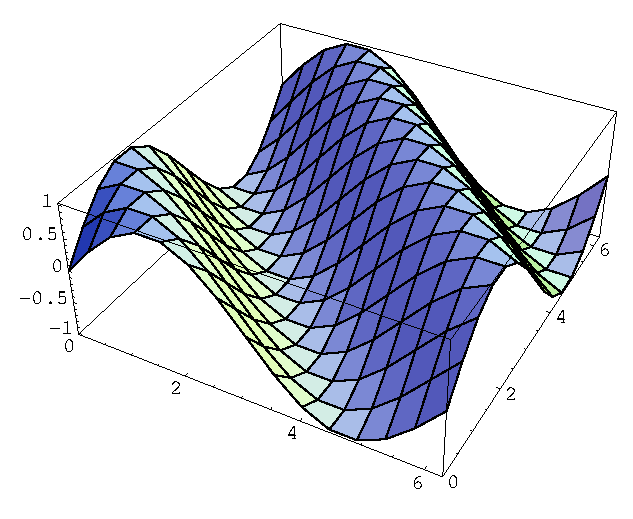
\includegraphics[width=0.6\textwidth]{calculus/vector/scafield}
  \end{center}
  \caption{A scalar field.}
  \label{figure scalar field}
\end{figure}


\begin{figure}[h!]
  \begin{center}
    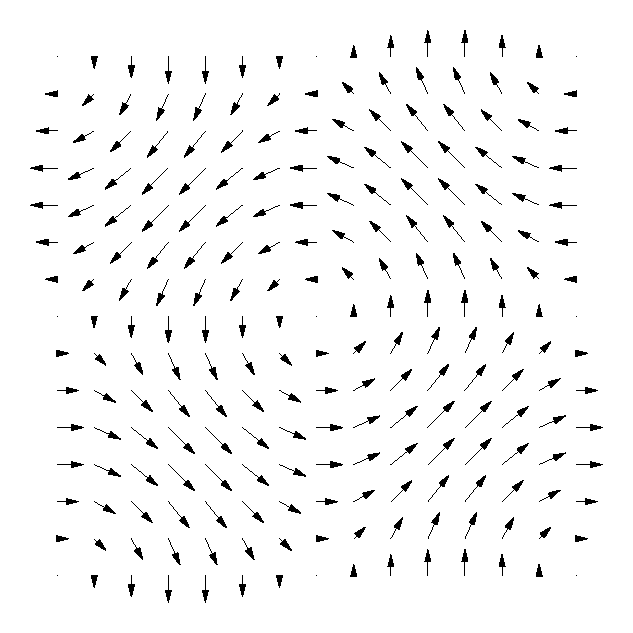
\includegraphics[width=0.6\textwidth]{calculus/vector/vecfield}
  \end{center}
  \caption{A vector field.}
  \label{figure vector field}
\end{figure}




\paragraph{Partial Derivatives of Scalar Fields.}
\index{partial derivative}
Consider a scalar field $u(\mathbf{x})$.  The \textit{partial derivative}
of $u$ with respect to $x_k$ is the derivative of $u$ in which $x_k$ is 
considered to be a variable and the remaining arguments are considered to be 
parameters.  The partial derivative is denoted 
$\frac{\partial}{\partial x_k} u(\mathbf{x})$, $\frac{\partial u}{\partial x_k}$ 
or $u_{x_k}$ and is defined
\[
\frac{\partial u}{\partial x_k} \equiv \lim_{\Delta x \to 0}
\frac{u(x_1, \ldots, x_k + \Delta x, \ldots, x_n) 
  - u(x_1, \ldots, x_k, \ldots, x_n)}{\Delta x}.
\]
Partial derivatives have the 
same differentiation formulas as ordinary derivatives.  

Consider a scalar field in $\mathbb{R}^3$, $u(x, y, z)$.
Higher derivatives of $u$ are denoted:
\begin{align*}
  u_{x x} &\equiv \frac{\partial^2 u}{\partial x^2} \equiv \frac{\partial}{\partial x} \frac{\partial u}{\partial x}, \\
  u_{x y} &\equiv \frac{\partial^2 u}{\partial x \partial y} \equiv \frac{\partial}{\partial x} 
  \frac{\partial u}{\partial y}, \\
  u_{x x y z} &\equiv \frac{\partial^4 u}{\partial x^2 \partial y \partial z} \equiv \frac{\partial^2}{\partial x^2} 
  \frac{\partial}{\partial y} \frac{\partial u}{\partial z}.
\end{align*}
If $u_{x y}$ and $u_{y x}$ are continuous, then
\[
\frac{\partial^2 u}{\partial x \partial y} = \frac{\partial^2 u}{\partial y \partial x}.
\]
This is referred to as the \textit{equality of mixed partial derivatives}.






\paragraph{Partial Derivatives of Vector Fields.}
Consider a vector field $\mathbf{u}(\mathbf{x})$.  
The partial derivative of $\mathbf{u}$ with respect to $x_k$ 
is denoted $\frac{\partial}{\partial x_k} \mathbf{u}(\mathbf{x})$, $\frac{\partial \mathbf{u}}{\partial x_k}$ 
or $\mathbf{u}_{x_k}$ and is defined
\[
\frac{\partial \mathbf{u}}{\partial x_k} \equiv \lim_{\Delta x \to 0}
\frac{\mathbf{u}(x_1, \ldots, x_k + \Delta x, \ldots, x_n) 
  - \mathbf{u}(x_1, \ldots, x_k, \ldots, x_n)}{\Delta x}.
\]
Partial derivatives of vector fields have the 
same differentiation formulas as ordinary derivatives.  








\paragraph{Gradient.}
\index{gradient}
\index{del}
\index{nabla}
We introduce the vector differential operator,
\[
\nabla \equiv \frac{\partial}{\partial x_1} \mathbf{e}_1 + \cdots
+ \frac{\partial}{\partial x_n} \mathbf{e}_n,
\]
which is known as \textit{del} or \textit{nabla}.
In $\mathbb{R}^3$ it is
\[
\nabla \equiv \frac{\partial}{\partial x} \mathbf{i} + \frac{\partial}{\partial y} \mathbf{j}
+ \frac{\partial}{\partial z} \mathbf{k}.
\]
Let $u(\mathbf{x})$ be a differential scalar field.  The \textit{gradient}
of $u$ is,
\[
\nabla u \equiv \frac{\partial u}{\partial x_1} \mathbf{e}_1 + \cdots
+ \frac{\partial u}{\partial x_n} \mathbf{e}_n,
\]






\paragraph{Directional Derivative.}
\index{directional derivative}
Suppose you are standing on some terrain.  The slope of the ground in 
a particular direction is the \textit{directional derivative} of the
elevation in that direction.  Consider a differentiable scalar field,
$u(\mathbf{x})$.  The derivative of the function in the direction of the
unit vector $\mathbf{a}$ is the rate of change of the function in that 
direction.  Thus the directional derivative, $D_{\mathbf{a}} u$, is defined:
\begin{align*}
  D_{\mathbf{a}} u(\mathbf{x}) 
  &= \lim_{\epsilon \to 0} 
  \frac{u(\mathbf{x} + \epsilon \mathbf{a}) - u(\mathbf{x})}{\epsilon} \\
  &= \lim_{\epsilon \to 0} 
  \frac{u(x_1 + \epsilon a_1, \ldots, x_n + \epsilon a_n)
    - u(x_1, \ldots, x_n) }{\epsilon} \\
  &= \lim_{\epsilon \to 0} 
  \frac{ \left( u(\mathbf{x}) 
      + \epsilon a_1 u_{x_1}(\mathbf{x}) + \cdots
      + \epsilon a_n u_{x_n}(\mathbf{x}) 
      + \mathcal{O}(\epsilon^2) \right) - u(\mathbf{x}) }
  { \epsilon } \\
  &= a_1 u_{x_1}(\mathbf{x}) + \cdots + a_n u_{x_n}(\mathbf{x}) 
\end{align*}
\[
D_{\mathbf{a}} u(\mathbf{x}) = \nabla u(\mathbf{x}) \cdot \mathbf{a}.
\]




%% CONTINUE: describe implicit functions:
%% f(x, y) = 0 is a 1D curve in 2D space.
%% f(x, y, z) = 0, ....




\paragraph{Tangent to a Surface.}
The gradient, $\nabla f$, is orthogonal to the surface $f(\mathbf{x}) = 0$.
Consider a point $\boldsymbol{\xi}$ on the surface.  Let the differential 
$d \mathbf{r} = d x_1 \mathbf{e}_1 + \cdots d x_n \mathbf{e}_n$ lie in the tangent
plane at $\boldsymbol{\xi}$.  Then
\[
d f = \frac{\partial f}{\partial x_1}\,d x_1 + \cdots + \frac{\partial f}{\partial x_n} \,d x_n = 0
\]
since $f(\mathbf{x}) = 0$ on the surface.  Then
\begin{align*}
  \nabla f \cdot d \mathbf{r} 
  &= \left( \frac{\partial f}{\partial x_1} \mathbf{e}_1 + \cdots 
    + \frac{\partial f}{\partial x_n} \mathbf{e}_n \right) \cdot
  \left( d x_1 \mathbf{e}_1 + \cdots + d x_n \mathbf{e}_n \right) \\
  &= \frac{\partial f}{\partial x_1} \,d x_1 + \cdots + \frac{\partial f}{\partial x_n} \,d x_n \\
  &= 0
\end{align*}
Thus $\nabla f$ is orthogonal to the tangent plane and hence to the surface.





\begin{Example}
  Consider the paraboloid, $x^2 + y^2 - z = 0$.  We want to find the tangent
  plane to the surface at the point $(1,1,2)$.  The gradient is
  \[
  \nabla f = 2 x \mathbf{i} + 2 y \mathbf{j} - \mathbf{k}.
  \]
  At the point $(1,1,2)$ this is
  \[
  \nabla f(1,1,2) = 2 \mathbf{i} + 2 \mathbf{j} - \mathbf{k}.
  \]
  We know a point on the tangent plane, $(1,1,2)$, and the normal, 
  $\nabla f(1,1,2)$.  The equation of the plane is
  \begin{gather*}
    \nabla f(1,1,2) \cdot (x, y, z) = \nabla f(1,1,2) \cdot (1,1,2) \\
    \boxed{
      2 x + 2 y - z = 2
      }
  \end{gather*}
\end{Example}




The gradient of the function $f(\mathbf{x}) = 0$, $\nabla f(\mathbf{x})$, is in 
the direction of the maximum directional derivative.   The magnitude 
of the gradient, $|\nabla f(\mathbf{x})|$, is the value of the directional
derivative in that direction.  To derive this, note that
\[
D_{\mathbf{a}} f = \nabla f \cdot \mathbf{a} = |\nabla f| \cos \theta,
\]
where $\theta$ is the angle between $\nabla f$ and $\mathbf{a}$.
$D_{\mathbf{a}} f$ is maximum when $\theta = 0$, i.e. when $\mathbf{a}$ is 
the same direction as $\nabla f$.  In this direction, 
$D_{\mathbf{a}} f = |\nabla f|$.
To use the elevation example, $\nabla f$ points in the uphill direction and
$|\nabla f|$ is the uphill slope.





\begin{Example}
  Suppose that the two surfaces $f(\mathbf{x}) = 0$ and $g(\mathbf{x}) = 0$ 
  intersect at the point $\mathbf{x} = \boldsymbol{\xi}$.  What is the angle between
  their tangent planes at that point?  First we note that the angle between
  the tangent planes is by definition the angle between their normals.
  These normals are in the direction of $\nabla f(\boldsymbol{\xi})$ and 
  $\nabla g(\boldsymbol{\xi})$.  (We assume these are nonzero.)  The angle, $\theta$,
  between the tangent planes to the surfaces is
  \[
  \boxed{
    \theta = \arccos \left( \frac{ \nabla f(\boldsymbol{\xi}) \cdot \nabla g(\boldsymbol{\xi}) }
      { | \nabla f(\boldsymbol{\xi}) |\,| \nabla g(\boldsymbol{\xi}) | } \right).
    }
  \]
\end{Example}








\begin{Example}
  Let $u$ be the distance from the origin: 
  \[
  u(\mathbf{x}) = \sqrt{\mathbf{x} \cdot \mathbf{x}} = \sqrt{x_i x_i}.
  \]
  In three dimensions, this is
  \[
  u(x, y, z) = \sqrt{x^2 + y^2 + z^2}.
  \]
  The gradient of $u$, $\nabla(\mathbf{x})$, is a unit vector in the direction 
  of $\mathbf{x}$.  The gradient is:
  \[
  \nabla u(\mathbf{x})
  = \left\langle \frac{x_1}{ \sqrt{ \mathbf{x} \cdot \mathbf{x} } }, \ldots,
    \frac{x_n}{ \sqrt{ \mathbf{x} \cdot \mathbf{x} } } \right\rangle
  = \frac{ x_i \mathbf{e}_i }{ \sqrt{ x_j x_j } }.
  \]
  In three dimensions, we have
  \[
  \nabla u(x, y, z) = \left \langle
    \frac{x}{\sqrt{x^2 + y^2 + z^2}},
    \frac{y}{\sqrt{x^2 + y^2 + z^2}},
    \frac{z}{\sqrt{x^2 + y^2 + z^2}} \right \rangle.
  \]
  This is a unit vector because the sum of the squared components sums to unity.
  \[
  \nabla u \cdot \nabla u = 
  \frac{ x_i \mathbf{e}_i }{ \sqrt{ x_j x_j } } \cdot
  \frac{ x_k \mathbf{e}_k }{ \sqrt{ x_l x_l } }
  \frac{ x_i x_i }{ x_j x_j } = 1
  \]
  Figure~\ref{grad_dist} shows a plot of the vector field of $\nabla u$ in 
  two dimensions.
  \begin{figure}[h!]
    \begin{center}
      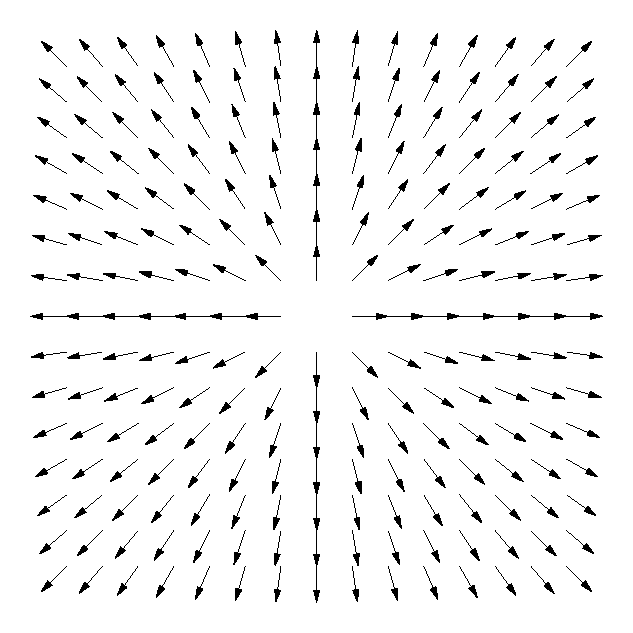
\includegraphics[width=0.6\textwidth]{calculus/vector/grad_dist}
    \end{center}
    \caption{The gradient of the distance from the origin.}
    \label{grad_dist}
  \end{figure}
\end{Example}












\begin{Example}
  Consider an ellipse.  An implicit equation of an ellipse is
  \[
  \frac{x^2}{a^2} + \frac{y^2}{b^2} = 1.
  \]
  We can also express an ellipse as $u(x,y) + v(x,y) = c$ 
  where $u$ and $v$ are the distance from the two foci.  That is, an ellipse 
  is the set of points such that the sum of the distances from the two foci is 
  a constant.  Let $\mathbf{n} = \nabla(u + v)$.  This is a vector which
  is orthogonal to the ellipse when evaluated on the surface.  Let $\mathbf{t}$
  be a unit tangent to the surface.  Since $\mathbf{n}$ and $\mathbf{t}$ are
  orthogonal,
  \begin{gather*}
    \mathbf{n} \cdot \mathbf{t} = 0 \\
    (\nabla u + \nabla v) \cdot \mathbf{t} = 0 \\
    \nabla u \cdot \mathbf{t} = \nabla v \cdot (- \mathbf{t}).
  \end{gather*}
  Since these are unit vectors, the angle between $\nabla u$ and $\mathbf{t}$
  is equal to the angle between $\nabla v$ and $-\mathbf{t}$.  In other
  words: If we draw rays from the foci to a point on the ellipse, the rays 
  make equal angles with the ellipse.   If the ellipse were a reflective 
  surface, a wave starting at one focus would be reflected from the ellipse and 
  travel to the other focus.  See Figure~\ref{ellipse and rays}.
  \begin{figure}[h!]
    \begin{center}
      \includegraphics[width=0.4\textwidth]{calculus/vector/ellipse}
    \end{center}
    \caption{An ellipse and rays from the foci.}
    \label{ellipse and rays}
  \end{figure}
  This result also holds for ellipsoids, $u(x,y, z) + v(x,y, z) = c$. 

  We see that an ellipsoidal dish could be used to collect spherical waves, 
  (waves emanating from a point).  If the dish is shaped so that the source
  of the waves is located at one foci and a collector is placed at the second,
  then any wave starting at the source and reflecting off the dish will travel
  to the collector.  See Figure~\ref{ellipse_dish}.
  \begin{figure}[h!]
    \begin{center}
      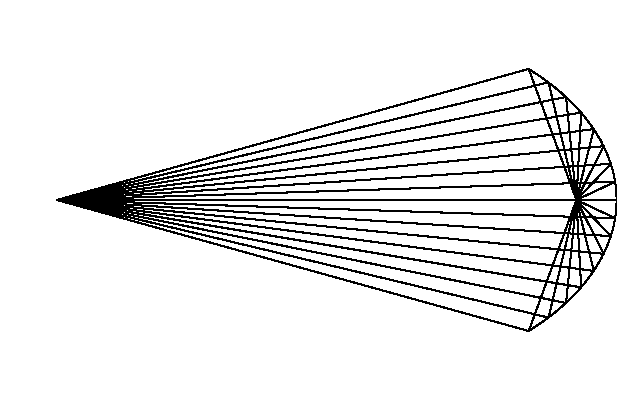
\includegraphics[width=0.8\textwidth]{calculus/vector/ellipse_dish}
    \end{center}
    \caption{An elliptical dish.}
    \label{ellipse_dish}
  \end{figure}
\end{Example}







\raggedbottom
%%=============================================================================
\pagebreak
\flushbottom
\section{Exercises}



%%-----------------------------------------------------------------------------
\begin{large}
  \noindent
  \textbf{Vector Functions}
\end{large}




%% Consider the parametric curve 
\begin{Exercise}
  \label{exercise parametric cos t/2 + sin t/2}
  Consider the parametric curve 
  \[
  \mathbf{r} = \cos \left( \frac{t}{2} \right) \mathbf{i} 
  + \sin \left( \frac{t}{2} \right) \mathbf{j}.
  \]
  Calculate $\frac{\dd \mathbf{r}}{\dd t}$ and
  $\frac{\dd^2 \mathbf{r}}{\dd t^2}$.  Plot the position and some velocity and
  acceleration vectors.

  \hintsolution{parametric cos t/2 + sin t/2}
\end{Exercise}





%% acceleration orthogonal to velocity
\begin{Exercise}
  \label{exercise constant speed acceleration orthogonal}
  Let $\mathbf{r}(t)$ be the position of an object moving with constant
  speed.  Show that the acceleration of the object is orthogonal to the
  velocity of the object.

  \hintsolution{constant speed acceleration orthogonal}
\end{Exercise}


%%-----------------------------------------------------------------------------
\begin{large}
  \noindent
  \textbf{Vector Fields}
\end{large}



%% Consider the surface given by $x^2 + y^2 - z = 0$.
\begin{Exercise}
  \label{exercise paraboloid x2 + y2 - z}
  Consider the paraboloid $x^2 + y^2 - z = 0$.  What is the angle
  between the two tangent planes that touch the surface at $(1,1,2)$ and
  $(1,-1,2)$?  What are the equations of the tangent planes at these points?

  \hintsolution{paraboloid x2 + y2 - z}
\end{Exercise}









%% Consider the paraboloid $x^2 + y^2 - z = 0$.
\begin{Exercise}
  \label{exercise paraboloid closest point}
  Consider the paraboloid $x^2 + y^2 - z = 0$.  What is the point on the
  paraboloid that is closest to $(1,0,0)$?

  \hintsolution{paraboloid closest point}
\end{Exercise}








\begin{Exercise}
  \label{exercise volume R rotate y}
  Consider the region $R$ defined by $x^2 + x y + y^2 \leq 9$.
  What is the volume of the solid obtained by rotating $R$ about the 
  $y$ axis?

  Is this the same as the volume of the solid obtained by rotating $R$ 
  about the $x$ axis?  Give geometric and algebraic explanations of this.

  \hintsolution{volume R rotate y}
\end{Exercise}







\begin{Exercise}
  \label{exercise cylinder intersect}
  Two cylinders of unit radius intersect at right angles as shown in 
  Figure~\ref{figure cylinder intersect}.  What is the volume of the solid
  enclosed by the cylinders?
  \begin{figure}[h!]
    \begin{center}
      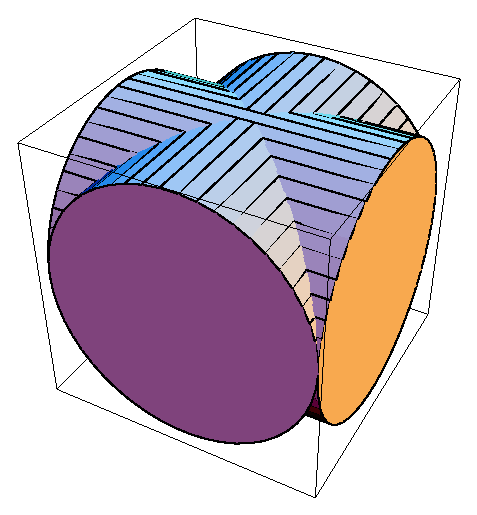
\includegraphics[width=0.3\textwidth]{calculus/vector/cylinderintersect}
    \end{center}
    \caption{Two cylinders intersecting.}
    \label{figure cylinder intersect}
  \end{figure}

  \hintsolution{cylinder intersect}
\end{Exercise}






\begin{Exercise}
  \label{exercise length area volume 1/x}
  Consider the curve $f(x) = 1/x$ on the interval $[1 \ldots \infty)$.  Let $S$ be
  the solid obtained by rotating $f(x)$ about the $x$ axis.  
  (See Figure~\ref{figure length area volume 1/x}.)
  Show that the length of $f(x)$ and the lateral area of $S$ are infinite.
  Find the volume of $S$.
  \footnote{You could fill $S$ with a finite amount of paint, but it would 
    take an infinite amount of paint to cover its surface.}
  \begin{figure}[h!]
    \begin{center}
      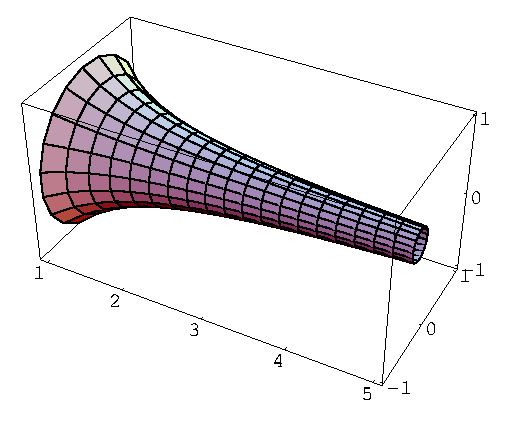
\includegraphics[width=0.4\textwidth]{calculus/vector/lav1x}
    \end{center}
    \caption{The rotation of $1/x$ about the $x$ axis.}
    \label{figure length area volume 1/x}
  \end{figure}

  \hintsolution{length area volume 1/x}
\end{Exercise}







\begin{Exercise}
  \label{exercise oil work}
  Suppose that a deposit of oil looks like a cone in the ground as 
  illustrated in Figure~\ref{figure oil work}.  Suppose that the oil has 
  a density of $800 \mathrm{kg} / \mathrm{m}^3$ and its vertical depth
  is $12 \mathrm{m}$.  How much work\footnote{
    Recall that $\mathrm{work} = \mathrm{force} \times \mathrm{distance}$
    and $\mathrm{force} = \mathrm{mass} \times \mathrm{acceleration}$. }
  would it take to get the oil to the surface.
  \begin{figure}[h!]
    \begin{center}
      \includegraphics[width=0.3\textwidth]{calculus/vector/oilwork}
    \end{center}
    \caption{The oil deposit.}
    \label{figure oil work}
  \end{figure}

  \hintsolution{oil work}
\end{Exercise}








\begin{Exercise}
  \label{exercise area volume sphere}
  Find the area and volume of a sphere of radius $R$ by integrating in 
  spherical coordinates.

  \hintsolution{area volume sphere}
\end{Exercise}






\raggedbottom
%%=============================================================================
\pagebreak
\flushbottom
\section{Hints}






%%-----------------------------------------------------------------------------
\begin{large}
  \noindent
  \textbf{Vector Functions}
\end{large}



%% Consider the parametric curve 
\begin{Hint}
  \label{hint parametric cos t/2 + sin t/2}
  Plot the velocity and acceleration vectors at regular intervals 
  along the path of motion.
\end{Hint}



%% acceleration orthogonal to velocity
\begin{Hint}
  \label{hint constant speed acceleration orthogonal}
  If $\mathbf{r}(t)$ has constant speed, then $| \mathbf{r}'(t) | = c$.
  The condition that the acceleration is orthogonal to the
  velocity can be stated mathematically in terms of the dot product,
  $\mathbf{r}''(t) \cdot \mathbf{r}'(t) = 0$.  Write the condition
  of constant speed in terms of a dot product and go from there.
\end{Hint}



%%-----------------------------------------------------------------------------
\begin{large}
  \noindent
  \textbf{Vector Fields}
\end{large}



%% Consider the surface given by $x^2 + y^2 - z = 0$.
\begin{Hint}
  \label{hint paraboloid x2 + y2 - z}
  The angle between two planes is the angle between the vectors orthogonal to 
  the planes.  The angle between the two vectors is
  \[
  \theta = \arccos \left( \frac{ \langle 2,2,-1 \rangle \cdot \langle 2,-2,-1 \rangle }
    { | \langle 2,2,-1 \rangle | | \langle 2,-2,-1 \rangle | } \right)
  \]
  The equation of a line orthogonal to $\mathbf{a}$ and passing 
  through the point $\mathbf{b}$ is $\mathbf{a} \cdot \mathbf{x} = \mathbf{a} \cdot \mathbf{b}$.
\end{Hint}



%% Consider the paraboloid $x^2 + y^2 - z = 0$.
\begin{Hint}
  \label{hint paraboloid closest point}
  Since the paraboloid is a differentiable surface, the normal to the surface
  at the closest point will be parallel to the vector from the closest
  point to $(1,0,0)$.  We can express this using the gradient and the 
  cross product.  If $(x,y,z)$ is the closest point on the paraboloid, then
  a vector orthogonal to the surface there is $\nabla f = \langle 2x,2y,-1 \rangle$.
  The vector from the surface to the point $(1,0,0)$ is $\langle 1-x,-y,-z \rangle$.
  These two vectors are parallel if their cross product is zero.
\end{Hint}



\begin{Hint}
  \label{hint volume R rotate y}
  CONTINUE  
\end{Hint}






\begin{Hint}
  \label{hint cylinder intersect}
  CONTINUE  
\end{Hint}








\begin{Hint}
  \label{hint length area volume 1/x}
  CONTINUE  
\end{Hint}





\begin{Hint}
  \label{hint oil work}
  Start with the formula for the work required to move the oil to 
  the surface.  Integrate over the mass of the oil.
  \[
  \mathrm{Work} = \int (\mathrm{acceleration})\,(\mathrm{distance})\,\dd (\mathrm{mass})
  \]
  Here (distance) is the distance of the differential of mass from the 
  surface.  The acceleration is that of gravity, $g$.
\end{Hint}





\begin{Hint}
  \label{hint area volume sphere}
  CONTINUE  
  %% Reference the Jacobian.
\end{Hint}







\raggedbottom
%%=============================================================================
\pagebreak
\flushbottom
\section{Solutions}






%%-----------------------------------------------------------------------------
\begin{large}
  \noindent
  \textbf{Vector Functions}
\end{large}



%% Consider the parametric curve 
\begin{Solution}
  \label{solution parametric cos t/2 + sin t/2}
  The velocity is 
  \[
  \mathbf{r}' = - \frac{1}{2} \sin \left( \frac{t}{2} \right) \mathbf{i} 
  + \frac{1}{2} \cos \left( \frac{t}{2} \right) \mathbf{j}.
  \]  
  The acceleration is 
  \[
  \mathbf{r}' = - \frac{1}{4} \cos \left( \frac{t}{2} \right) \mathbf{i} 
  - \frac{1}{4} \sin \left( \frac{t}{2} \right) \mathbf{j}.
  \]  
  See Figure~\ref{circleva} for plots of position, velocity and acceleration.

  \begin{figure}[h!]
    \begin{center}
      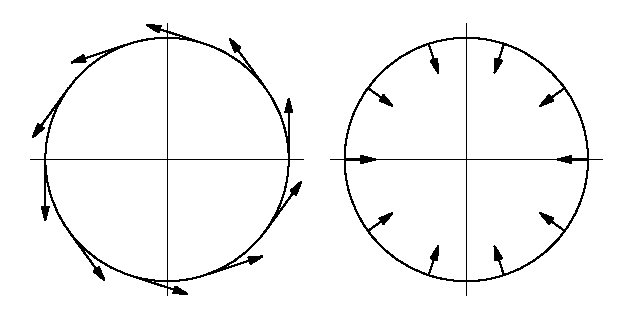
\includegraphics[width=0.8\textwidth]{calculus/vector/circleva}
    \end{center}
    \caption{A graph of position and velocity and of position and 
      acceleration.}
    \label{circleva}
  \end{figure}
\end{Solution}






%% acceleration orthogonal to velocity
\begin{Solution}
  \label{solution constant speed acceleration orthogonal}
  If $\mathbf{r}(t)$ has constant speed, then $| \mathbf{r}'(t) | = c$.
  The condition that the acceleration is orthogonal to the
  velocity can be stated mathematically in terms of the dot product,
  $\mathbf{r}''(t) \cdot \mathbf{r}'(t) = 0$.  Note that we can write the condition
  of constant speed in terms of a dot product, 
  \[
  \sqrt{ \mathbf{r}'(t) \cdot \mathbf{r}'(t) } = c,
  \]
  \[
  \mathbf{r}'(t) \cdot \mathbf{r}'(t) = c^2.
  \]
  Differentiating this equation yields,
  \[
  \mathbf{r}''(t) \cdot \mathbf{r}'(t) + \mathbf{r}'(t) \cdot \mathbf{r}''(t) = 0
  \]
  \[
  \mathbf{r}''(t) \cdot \mathbf{r}'(t) = 0.
  \]
  This shows that the acceleration is orthogonal to the velocity.
\end{Solution}






%%-----------------------------------------------------------------------------
\begin{large}
  \noindent
  \textbf{Vector Fields}
\end{large}




%% Consider the surface given by $x^2 + y^2 - z = 0$.
\begin{Solution}
  \label{solution paraboloid x2 + y2 - z}
  The gradient, which is orthogonal to the surface when evaluated there is
  $\nabla f = 2x \mathbf{i} + 2 y \mathbf{j} - \mathbf{k}$.  
  $2 \mathbf{i} + 2 \mathbf{j} - \mathbf{k}$ and $2 \mathbf{i} - 2 \mathbf{j} - \mathbf{k}$ are
  orthogonal to the paraboloid, (and hence the tangent planes), at the points 
  $(1,1,2)$ and $(1,-1,2)$, respectively.  The angle between the tangent
  planes is the angle between the vectors orthogonal to the planes.  The 
  angle between the two vectors is
  \[
  \theta = \arccos \left( \frac{ \langle 2,2,-1 \rangle \cdot \langle 2,-2,-1 \rangle }
    { | \langle 2,2,-1 \rangle | | \langle 2,-2,-1 \rangle | } \right)
  \]
  \[
  \boxed{
    \theta = \arccos \left( \frac{1}{9} \right)
    \approx 1.45946.
    }
  \]
  Recall that the equation of a line orthogonal to $\mathbf{a}$ and passing 
  through the point $\mathbf{b}$ is $\mathbf{a} \cdot \mathbf{x} = \mathbf{a} \cdot \mathbf{b}$.
  The equations of the tangent planes are
  \[
  \langle 2,\pm 2,-1 \rangle \cdot \langle x,y,z \rangle 
  = \langle 2,\pm 2,-1 \rangle \cdot \langle 1,\pm 1,2 \rangle,
  \]
  \[
  \boxed{
    2 x \pm 2 y - z = 2.
    }
  \]
  The paraboloid and the tangent planes are shown in Figure~\ref{paratp}.

  \begin{figure}[h!]
    \begin{center}
      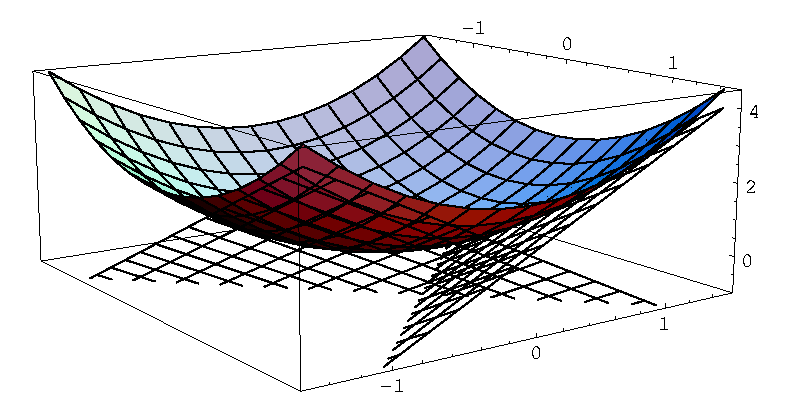
\includegraphics[width=0.4\textwidth]{calculus/vector/paratp}
    \end{center}
    \caption{Paraboloid and two tangent planes.}
    \label{paratp}
  \end{figure}
\end{Solution}








%% Consider the paraboloid $x^2 + y^2 - z = 0$.
\begin{Solution}
  \label{solution paraboloid closest point}
  Since the paraboloid is a differentiable surface, the normal to the surface
  at the closest point will be parallel to the vector from the closest
  point to $(1,0,0)$.  We can express this using the gradient and the 
  cross product.  If $(x,y,z)$ is the closest point on the paraboloid, then
  a vector orthogonal to the surface there is $\nabla f = \langle 2x,2y,-1 \rangle$.
  The vector from the surface to the point $(1,0,0)$ is $\langle 1-x,-y,-z \rangle$.
  These two vectors are parallel if their cross product is zero,
  \[
  \langle 2x,2y,-1 \rangle \times \langle 1-x,-y,-z \rangle 
  = \langle -y - 2 y z, -1 + x + 2 x z, -2 y \rangle = \mathbf{0}.
  \]
  This gives us the three equations,
  \begin{align*}
    -y - 2 y z &= 0, \\
    -1 + x + 2 x z &= 0, \\
    -2 y &= 0.
  \end{align*}
  The third equation requires that $y = 0$.  The first equation then becomes
  trivial and we are left with the second equation,
  \[
  -1 + x + 2 x z = 0.
  \]
  Substituting $z = x^2 + y^2$ into this equation yields,
  \[
  2 x^3 + x - 1 = 0.
  \]
  The only real valued solution of this polynomial is
  \[
  x = \frac{ 6^{-2/3} \left( 9 + \sqrt{87} \right)^{2/3} - 6^{-1/3} }
  { \left( 9 + \sqrt{87} \right)^{1/3} }
  \approx 0.589755.
  \]
  Thus the closest point to $(1,0,0)$ on the paraboloid is
  \[
  \left( \frac{ 6^{-2/3} \left( 9 + \sqrt{87} \right)^{2/3} - 6^{-1/3} }
    { \left( 9 + \sqrt{87} \right)^{1/3} }, 0,
    \left( \frac{ 6^{-2/3} \left( 9 + \sqrt{87} \right)^{2/3} - 6^{-1/3} }
      { \left( 9 + \sqrt{87} \right)^{1/3} } \right)^2 \right)
  \approx (0.589755, 0, 0.34781).
  \]
  The closest point is shown graphically in Figure~\ref{paracp}.

  \begin{figure}[h!]
    \begin{center}
      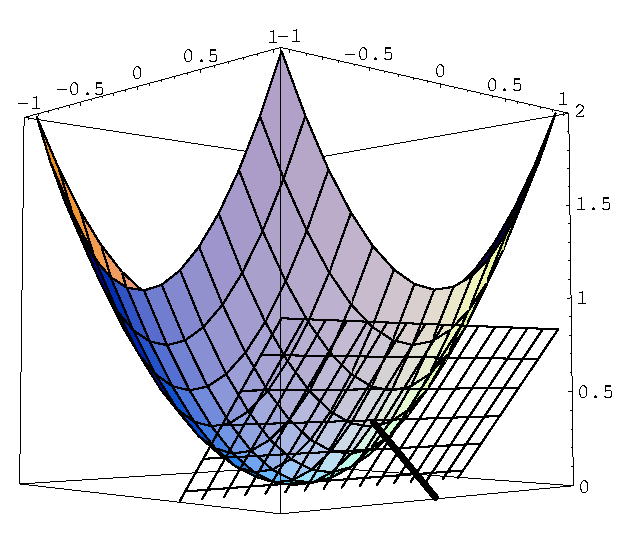
\includegraphics[width=0.4\textwidth]{calculus/vector/paracp}
    \end{center}
    \caption{Paraboloid, tangent plane and line connecting $(1,0,0)$ to
      the closest point.}
    \label{paracp}
  \end{figure}
\end{Solution}









\begin{Solution}
  \label{solution volume R rotate y}
  We consider the region $R$ defined by $x^2 + x y + y^2 \leq 9$.  The boundary
  of the region is an ellipse.  (See Figure~\ref{figure x2xyy29} for the 
  ellipse and the solid obtained by rotating the region.)
  \begin{figure}[h!]
    \begin{center}
      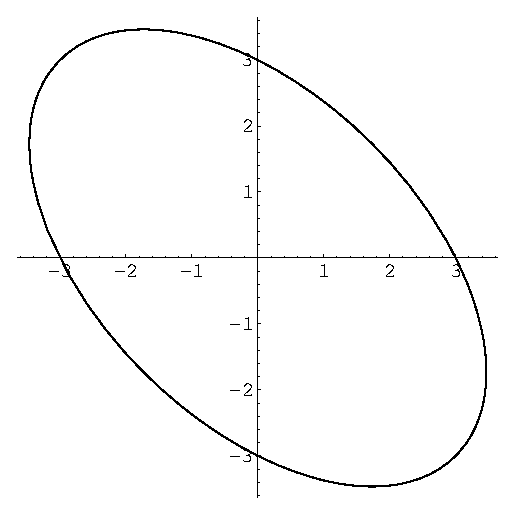
\includegraphics[width=0.4\textwidth]{calculus/vector/x2xyy29}
      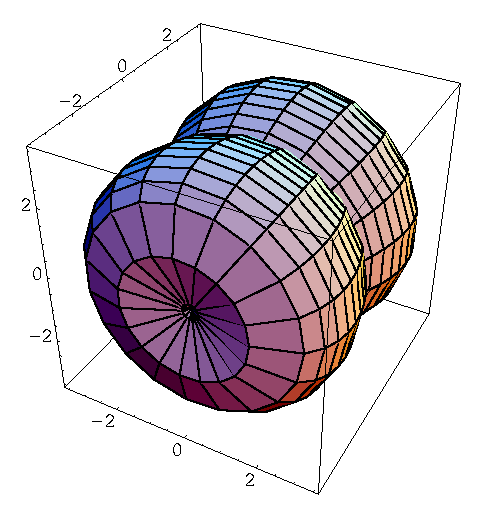
\includegraphics[width=0.4\textwidth]{calculus/vector/x2xyy29solid}
    \end{center}
    \caption{The ellipse and the solid.}
    \label{figure x2xyy29}
  \end{figure}
  Note that in rotating the region about the $y$ axis, only the portions in
  the second and fourth quadrants make a contribution.  Since the solid is
  symmetric across the $x z$ plane, we will find the volume of the top half
  and then double this to get the volume of the whole solid.  Now we consider
  rotating the region in the second quadrant about the $y$ axis. In the 
  equation for the ellipse, $x^2 + x y + y^2 = 9$, we solve for $x$.
  \[
  x = \frac{1}{2} \left( -y \pm \sqrt{3} \sqrt{12 - y^2} \right)
  \]
  In the second quadrant, the curve $(-y - \sqrt{3} \sqrt{12 - y^2})/2$
  is defined on $y \in [0 \ldots \sqrt{12}]$ and the curve 
  $(-y - \sqrt{3} \sqrt{12 - y^2})/2$ is defined on $y \in [3 \ldots \sqrt{12}]$.
  (See Figure~\ref{figure x2xyy29q2}.  The former is shown in red and 
  the latter in green.)
  \begin{figure}[h!]
    \begin{center}
      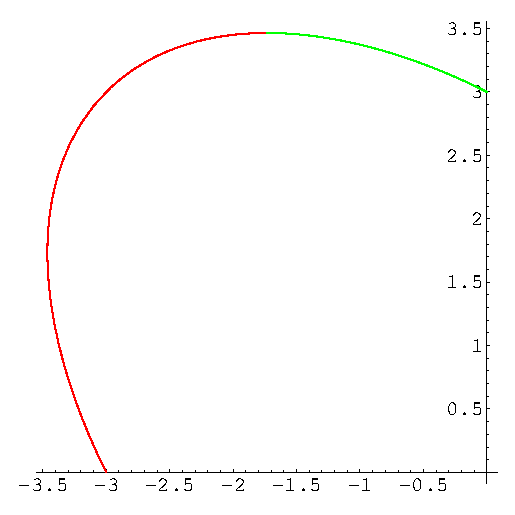
\includegraphics[height=2.5in]{calculus/vector/x2xyy29q2}
    \end{center}
    \caption{The two portions of the curve.}
    \label{figure x2xyy29q2}
  \end{figure}
  We find the volume obtained by rotating the first curve and subtract the 
  volume from rotating the second curve.
  \begin{gather*}
    V = 2 \left( \int_0^{\sqrt{12}} \pi \left( 
        \frac{-y - \sqrt{3} \sqrt{12 - y^2}}{2} \right)^2 \,\dd y
      - \int_3^{\sqrt{12}} \pi \left( 
        \frac{-y + \sqrt{3} \sqrt{12 - y^2}}{2} \right)^2 \,\dd y \right)
    \\
    V = \frac{\pi}{2} \left( \int_0^{\sqrt{12}} \left( 
        y + \sqrt{3} \sqrt{12 - y^2} \right)^2 \,\dd y
      - \int_3^{\sqrt{12}}  \left( 
        -y + \sqrt{3} \sqrt{12 - y^2} \right)^2 \,\dd y \right)
    \\
    V = \frac{\pi}{2} \left( \int_0^{\sqrt{12}} \left( 
        -2 y^2 + \sqrt{12} y \sqrt{12 - y^2} + 36 \right) \,\dd y
      - \int_3^{\sqrt{12}} \left( 
        -2 y^2 - \sqrt{12} y \sqrt{12 - y^2} + 36 \right) \,\dd y \right)
    \\
    V = \frac{\pi}{2} \left( 
      \left[ - \frac{2}{3} y^3 
        - \frac{2}{\sqrt{3}} \left( 12 - y^2 \right)^{3/2} + 36 y \right]_0^{\sqrt{12}}
      - \left[ - \frac{2}{3} y^3 
        + \frac{2}{\sqrt{3}} \left( 12 - y^2 \right)^{3/2} + 36 y \right]_3^{\sqrt{12}}
    \right)
    \\
    \boxed{
      V = 72 \pi
      }
  \end{gather*}

  Now consider the volume of the solid obtained by rotating $R$ 
  about the $x$ axis?  This as the same as the volume of the solid obtained
  by rotating $R$ about the $y$ axis.  Geometrically we know this because
  $R$ is symmetric about the line $y = x$.

  Now we justify it algebraically.  Consider the phrase: Rotate the region
  $x^2 + x y + y^2 \leq 9$ about the $x$ axis.  We formally swap $x$ and $y$ to 
  obtain: Rotate the region $y^2 + y x + x^2 \leq 9$ about the $y$ axis.  Which
  is the original problem.
\end{Solution}








\begin{Solution}
  \label{solution cylinder intersect}
  We find of the volume of the intersecting cylinders by summing the volumes
  of the two cylinders and then subracting the volume of their intersection.
  The volume of each of the cylinders is $2 \pi$.  The intersection is shown
  in Figure~\ref{figure intersection cylinders}.  If we slice this solid
  along the plane $z = \mathrm{const}$ we have a square with side length
  $2 \sqrt{1 - z^2}$.  The volume of the intersection of the cylinders is 
  \[
  \int_{-1}^1 4 \left( 1 - z^2 \right) \,\dd z.
  \]
  \begin{figure}[h!]
    \begin{center}
      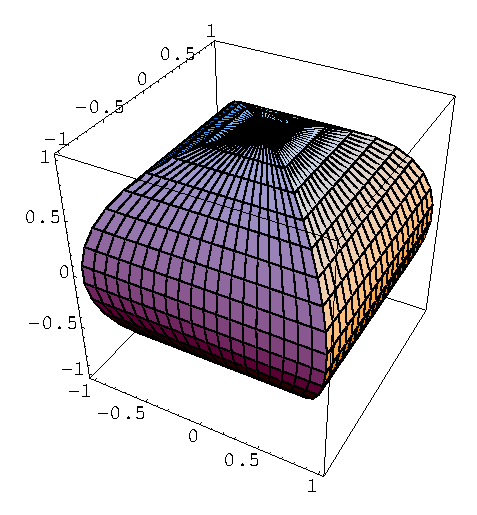
\includegraphics[width=0.4\textwidth]{calculus/vector/cylinderintersection}
    \end{center}
    \caption{The intersection of the two cylinders.}
    \label{figure intersection cylinders}
  \end{figure}
  We compute the volume of the intersecting cylinders.
  \begin{gather*}
    V = 2 (2 \pi) - 2 \int_0^1 4 \left( 1 - z^2 \right) \,\dd z
    \\
    \boxed{
      V = 4 \pi - \frac{16}{3}
      }
  \end{gather*}
\end{Solution}





\begin{Solution}
  \label{solution length area volume 1/x}
  The length of $f(x)$ is 
  \[
  L = \int_1^\infty \sqrt{1 + 1/x^2} \,\dd x.
  \]
  Since $\sqrt{1 + 1/x^2} > 1/x$, the integral diverges.  The length is 
  infinite.

  We find the area of $S$ by integrating the length of circles.
  \[
  A = \int_1^\infty \frac{2 \pi}{x} \,\dd x
  \]
  This integral also diverges.  The area is infinite.

  Finally we find the volume of $S$ by integrating the area of disks.
  \[
  V = \int_1^\infty \frac{\pi}{x^2} \,\dd x = \left[ - \frac{\pi}{x} \right]_1^\infty = \pi
  \]
\end{Solution}




\begin{Solution}
  \label{solution oil work}
  First we write the formula for the work required to move the oil to 
  the surface.  We integrate over the mass of the oil.
  \[
  \mathrm{Work} = \int (\mathrm{acceleration})\,(\mathrm{distance})\,\dd (\mathrm{mass})
  \]
  Here (distance) is the distance of the differential of mass from the 
  surface.  The acceleration is that of gravity, $g$.  The differential
  of mass can be represented an a differential of volume time the density 
  of the oil, $800\, \mathrm{kg} / \mathrm{m}^3$.
  \[
  \mathrm{Work} = \int 800 g (\mathrm{distance}) \,\dd (\mathrm{volume})
  \]

  We place the coordinate axis so that $z = 0$ coincides with the bottom 
  of the cone.  The oil lies between $z = 0$ and $z = 12$.  The cross
  sectional area of the oil deposit at a fixed depth is $\pi z^2$.  Thus the 
  differential of volume is $\pi\, z^2\, \dd z$.
  This oil must me raised a distance of $24 - z$.
  \begin{gather*}
    W = \int_0^{12} 800\, g\, (24 - z)\, \pi\, z^2\, \dd z
    \\
    W = 6912000 g \pi
    \\
    \boxed{
      W \approx 2.13 \times 10^8 \, \frac{ \mathrm{kg}\, \mathrm{m}^2 }{ \mathrm{s}^2 }
      }
  \end{gather*}
\end{Solution}



\begin{Solution}
  \label{solution area volume sphere}
  %% CONTINUE Reference the Jacobian.
  The Jacobian in spherical coordinates is $r^2 \sin \phi$.
  \begin{align*}
    \mathrm{area} 
    &= \int_0^{2 \pi} \int_0^\pi R^2 \sin \phi \,\dd \phi \,\dd \theta
    \\
    &= 2 \pi R^2 \int_0^\pi \sin \phi \,\dd \phi
    \\
    &= 2 \pi R^2 [- \cos \phi]_0^\pi
  \end{align*}
  \[
  \boxed{
    \mathrm{area} = 4 \pi R^2
    }
  \]
  \begin{align*}
    \mathrm{volume} 
    &= \int_0^R \int_0^{2 \pi} \int_0^\pi r^2 \sin \phi \,\dd \phi \,\dd \theta \,\dd r
    \\
    &= 2 \pi \int_0^R \int_0^\pi r^2 \sin \phi \,\dd \phi \,\dd r
    \\
    &= 2 \pi \left[ \frac{r^3}{3} \right]_0^R [- \cos \phi ]_0^\pi
  \end{align*}
  \[
  \boxed{
    \mathrm{volume} = \frac{4}{3} \pi R^3
    }
  \]
\end{Solution}


\raggedbottom
%%=============================================================================
\pagebreak
\flushbottom
\section{Quiz}


\begin{QuizProblem}
  \label{quiz problem distance plane x+2y+3z=4}
  What is the distance from the origin to the plane $x + 2 y + 3 z = 4$?

  \quizsolution{distance plane x+2y+3z=4}
\end{QuizProblem}


\begin{QuizProblem}
  \label{quiz problem bead on a wire}
  A bead of mass $m$ slides frictionlessly on a wire determined
  parametrically by $\mathbf{w}(s)$.  The bead moves under the force of
  gravity.  What is the acceleration of the bead as a function of the
  parameter $s$?

  \quizsolution{bead on a wire}
\end{QuizProblem}









\raggedbottom
%%=============================================================================
\pagebreak
\flushbottom
\section{Quiz Solutions}


\begin{QuizSolution}
  \label{quiz solution distance plane x+2y+3z=4}
  Recall that the equation of a plane is 
  $\mathbf{x} \cdot \mathbf{n} = \mathbf{a} \cdot \mathbf{n}$ where $\mathbf{a}$ 
  is a point in the plane and $\mathbf{n}$ is normal to the plane.  
  We are considering the plane $x + 2 y + 3 z = 4$.  A normal to the 
  plane is $\langle 1, 2, 3 \rangle$.  The unit normal is
  \[
  \mathbf{n} = \frac{1}{\sqrt{15}} \langle 1, 2, 3 \rangle.
  \]
  By substituting in $x = y = 0$, we see that a point in the plane is
  $\mathbf{a} = \langle 0, 0, 4/3 \rangle$.  The distance of the plane from the origin is
  $\mathbf{a} \cdot \mathbf{n} = \frac{4}{\sqrt{15}}$.
\end{QuizSolution}


\begin{QuizSolution}
  \label{quiz solution bead on a wire}
  The force of gravity is $- g \mathbf{k}$.  The unit tangent to the wire is 
  $\mathbf{w}'(s) / |\mathbf{w}'(s)|$.    The component of the gravitational 
  force in the tangential direction is 
  $- g \mathbf{k} \cdot \mathbf{w}'(s) / | \mathbf{w}'(s) |$.
  Thus the acceleration of the bead is
  \[
  - \frac{g \mathbf{k} \cdot \mathbf{w}'(s)}{m | \mathbf{w}'(s) |}.
  \]
\end{QuizSolution}




\raggedbottom


